%Template generated by Ben Manning
%Purdue University
%btmannin@purdue.edu
%Last modified: 7/7/2021


\documentclass[notitlepage, 12pt]{report}  %The document class will setup a lot of basic formatting.  Report class will start with justifying paragraphs setup your different types of sections.

%Different packages allow you to add more functions that will make your time in LaTeX easier.
\usepackage{amsmath}
\usepackage{graphicx}
\usepackage{caption}
\usepackage{url}
\usepackage{circuitikz} % circuit drawer

\graphicspath{{./images}}

%\usepackage{biblatex} %Imports biblatex package
\usepackage[style=numeric]{biblatex}
\addbibresource{bib.bib}

\usepackage[top=2cm, bottom=2cm, left=2cm, right=2cm]{geometry}

\title{Experiment 4 Report}

\begin{document}
%Everything needs to begin and end.  


\begin{center}
\large \textbf{Experiment 4 Report} \\ %\large and \small can help make text sizes vary throughout your document.
%\textbf will bold the text that is in the curly brackets
\small 
Andrew Lykken\\
Anna Kishnani\\
February 9 2023\\
Section 004 (Abraham Yakisan)\\
%\rule{500pt}{.1pt} 

\end{center}

% space between tite and abstract
\vspace{4in}


\begin{abstract}

In this experiment, an ALD1106 Dual matched pair n-channel MOSFET array chip is used to create a current mirror circuit and 
an inverting amplifier. In the current mirror application, the current can be set based on various voltages, as described and equated 
later in this document. The inverting amplifier can have a desired gain and frequency response, and these values can manipulate what voltages 
are needed where, and thus, what parts to use in the circuit. We were sucessful in creating both of these circuits, testing extensively, and 
evaluating our performance through mathematical and graphical interpretation.

\end{abstract}

\newpage

\section*{Task 1} %Each task has a section including (but not limited to) Objective, 
% Procedure, Results / Calculations, Conclusions


\subsection*{Objective}

\indent\indent The objective of this task is to design and build a current mirror circuit using the ALD1106 
dual matched pair n-channel MOSFET array.\\

\subsection*{Procedure}

\textbf{Step 1}

The circuit below was built:

\begin{center}
    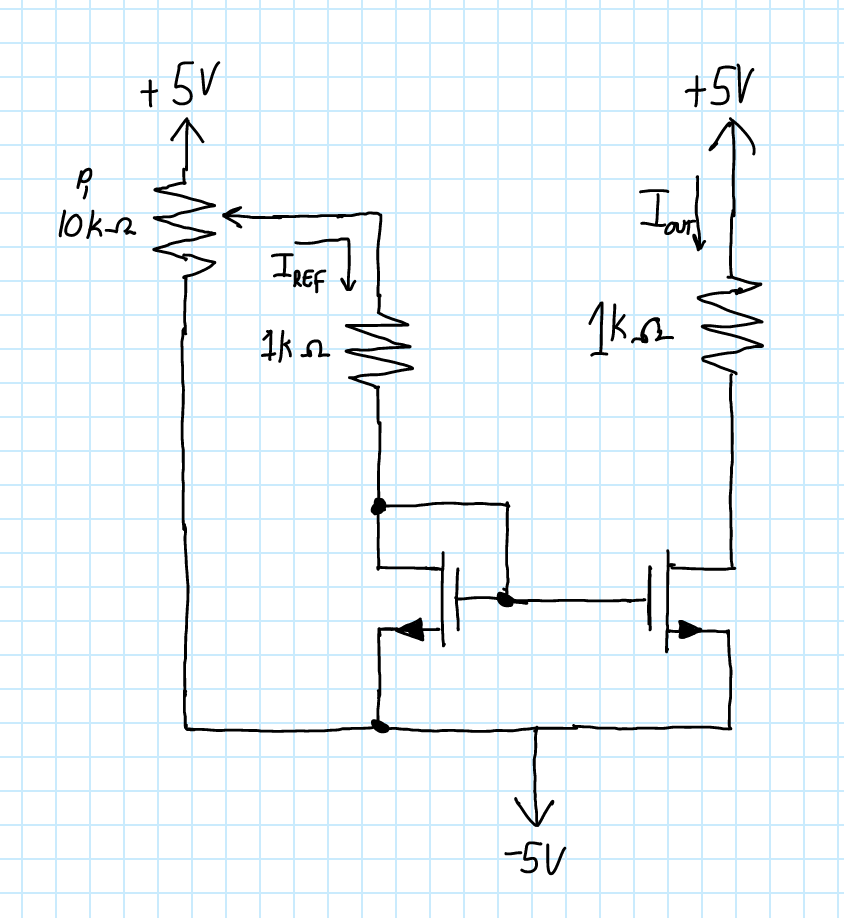
\includegraphics[scale=0.3]{currentmirror.png}
\end{center}

\textbf{Step 2}

The current $I_{OUT}$ was plotted against $I_{REF}$ between $I_{REF}$ = 0.1 mA and 2.5 mA. This was done by 
measuring the voltage across $R_{REF}$ and $R_{TEST}$ respectively, and computing the current through each 
using Ohm's law.\\

\textbf{Step 3}

The reference current was set to 1.34 mA, as calculated from prelab question 2. The gate-source ($v_{GS}$) and drain-source ($v_{DS}$) voltages were 
measured for each transistor. \\

\newpage

\subsection*{Results / Calculations}

\textbf{Step 2}
The following plot was created:

\begin{center}
    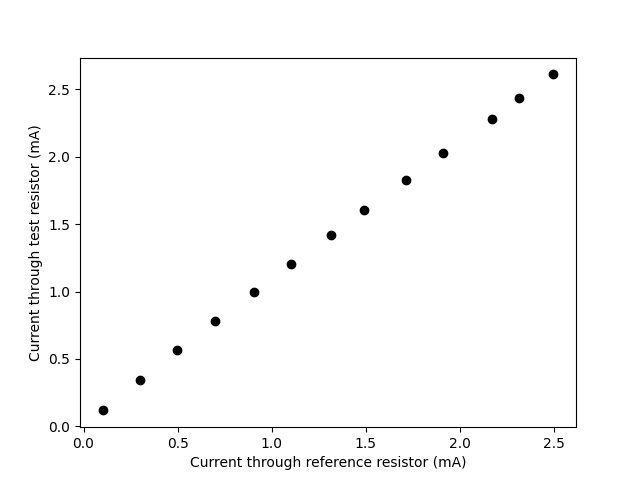
\includegraphics[scale=0.6]{current_plot.png}
\end{center}

The plot shows that the current going through the reference resistor is very close to the current going through the test resistor, meaning 
the current mirror is working correctly. The average difference in current between the two resistors is 0.092 mA. \\

\textbf{Step 3}
The measured voltages from each transistor were: \\

Q1 (Left transistor) : $v_{GS}$ = 2.5897V , $v_{DS}$ = 2.5899V \\

Q2 (Right transistor): $v_{GS}$ = 2.5901V , $v_{DS}$ = 8.5536V \\

\subsection*{Conclusions}

\indent\indent In this task, we created a current mirror circuit that matched the current from one transistor to another. 
This circuit worked very well, as shown by the plot of current values.

\newpage

\section*{Task 2}

\subsection*{Objective}
\indent\indent The objective of this task is to create an inverting amplifier with specifications determined in the lab manual. 

\subsection*{Procedure}

\textbf{Step 0 (Prelab Question 2)} 
The values of $R_1$, $R_2$, $R_D$, and $I_{BIAS}$ were calculated such that the gain $A_v$ is -4, the DC output voltage is around 1V, 
and the minimum output voltage was -1V. Additionally, $R_1$ || $R_2$ must be greater than 100k$\Omega$. \\

\textbf{Step 1}
The values of $C_1$ and $C_2$ were calculated such that the -3dB point of the frequency response would be at 30 Hz. \\

\textbf{Step 2}
The following circuit was built using the values calculated above:

\begin{center}
    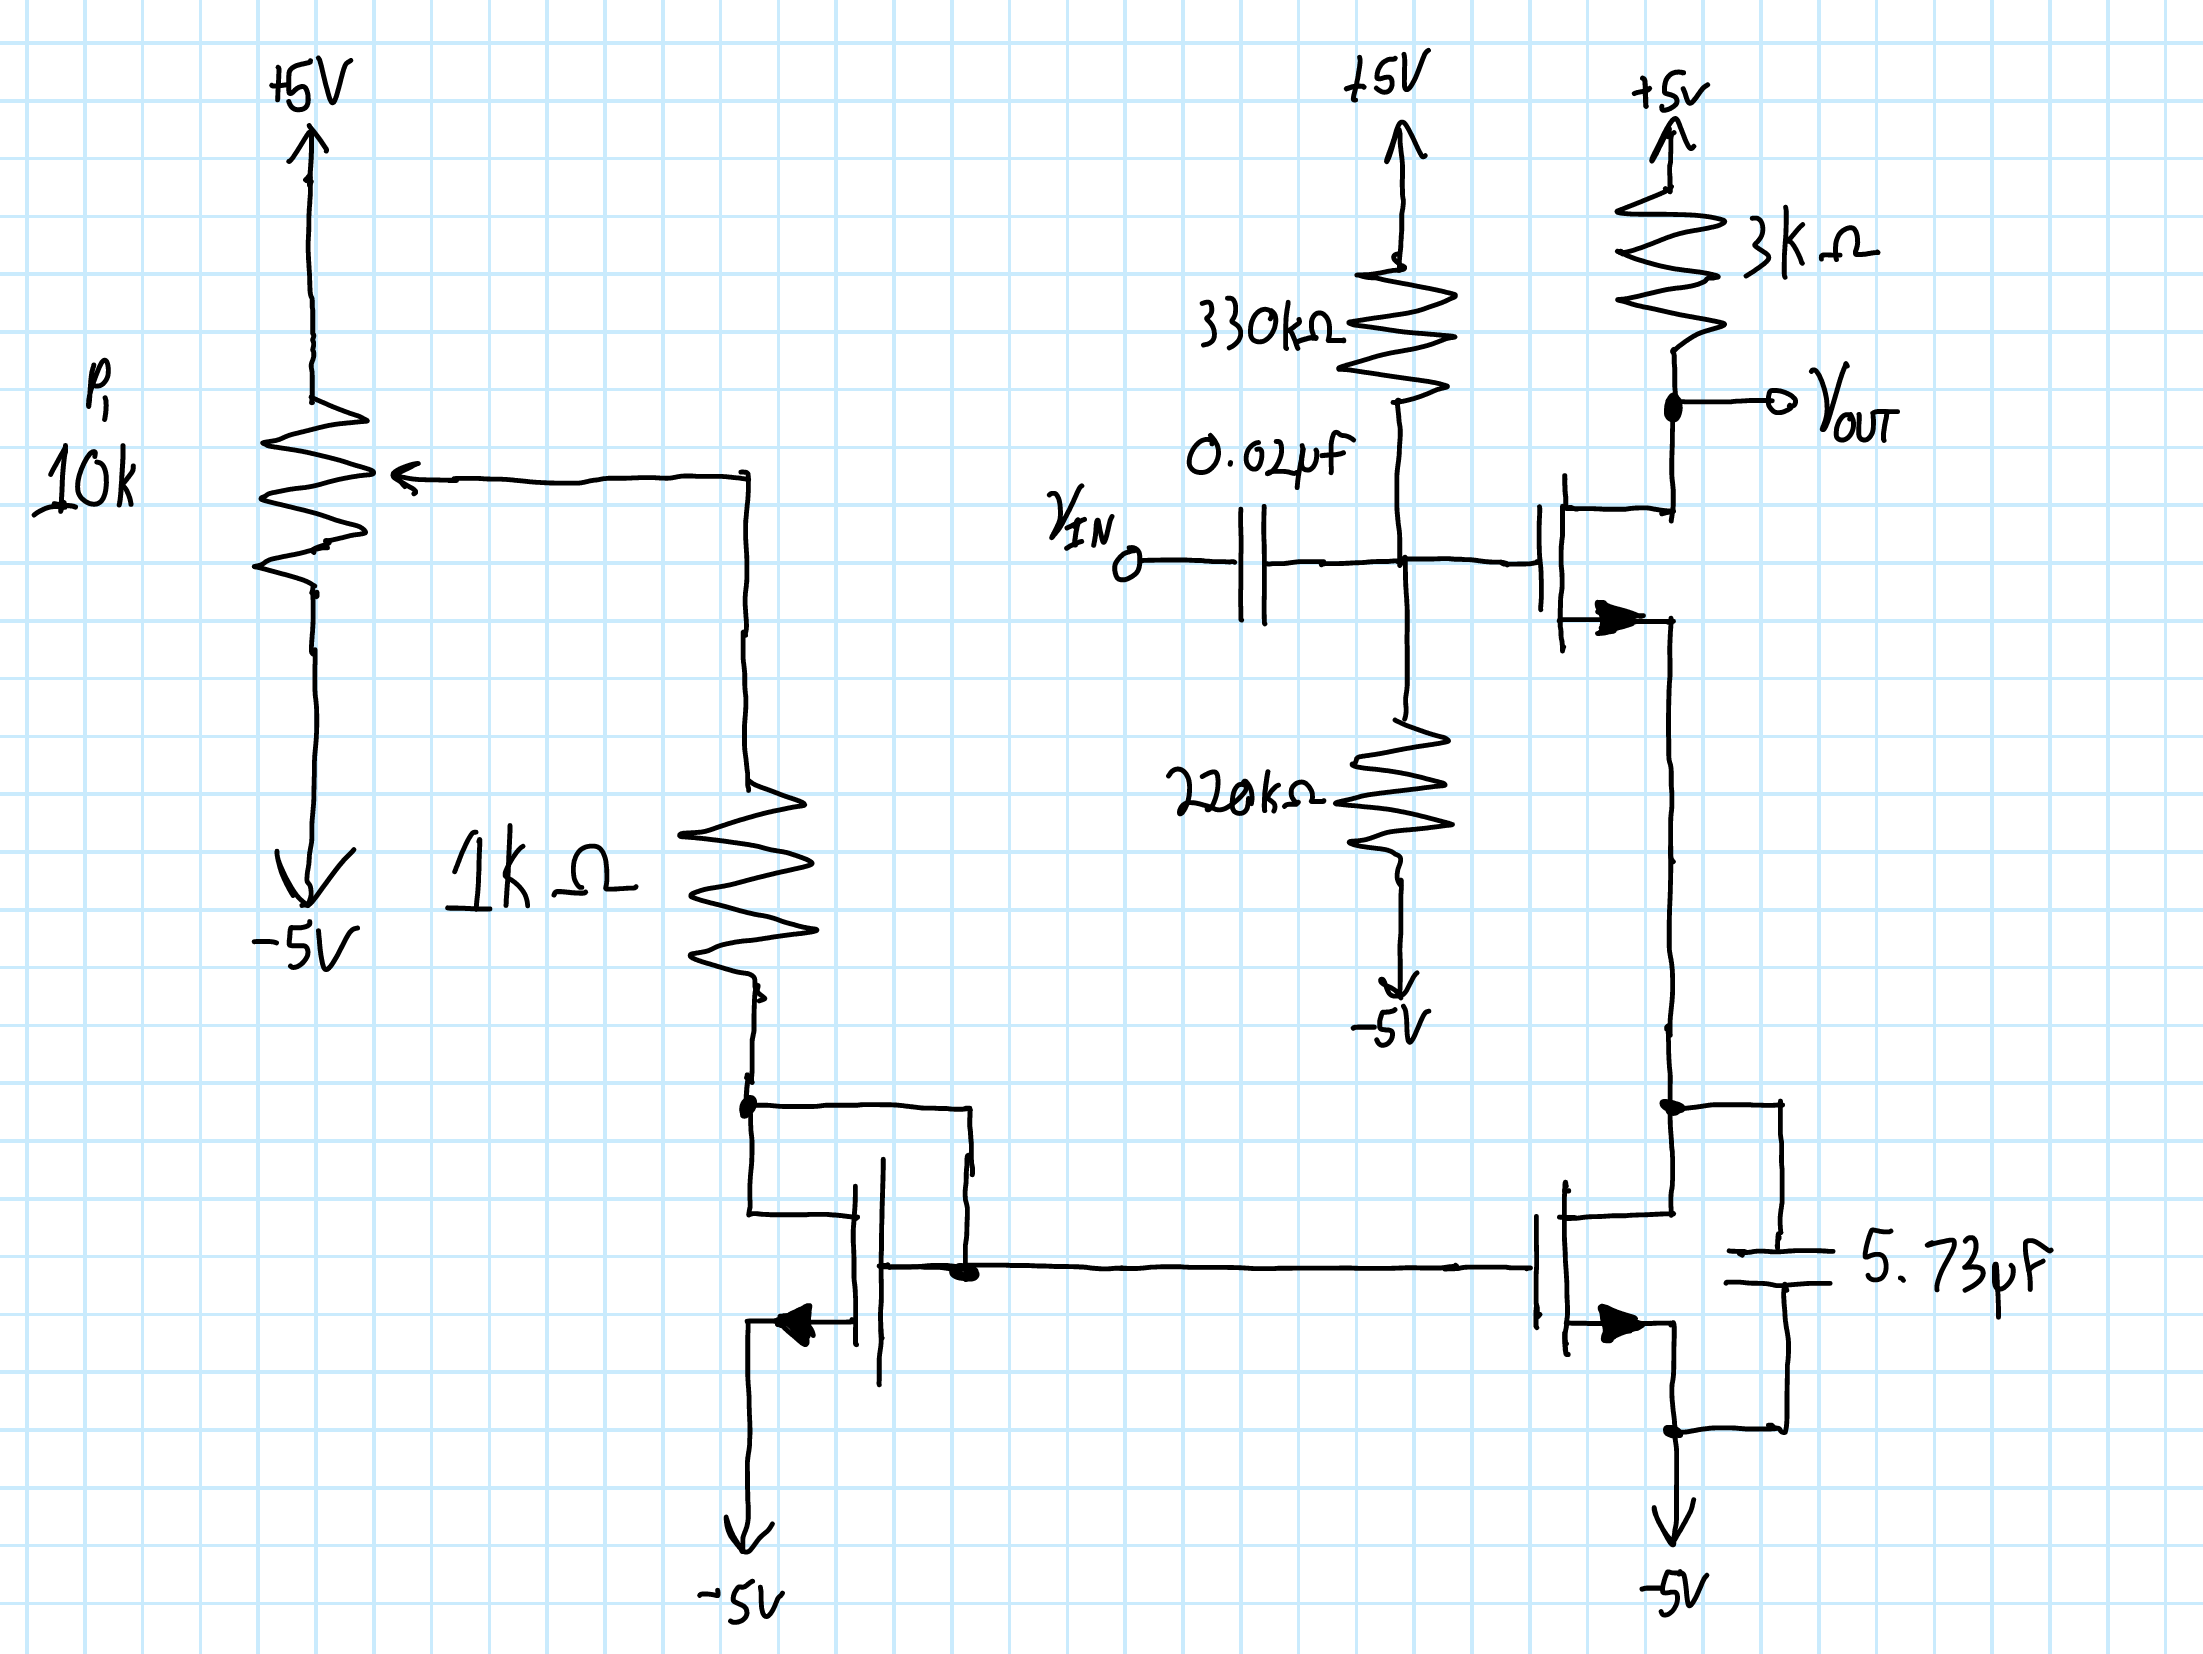
\includegraphics[scale=0.17]{task2.png}
\end{center}

\textbf{Step 3}
The AC input $v_{IN}$ was set to 0V, and adjust the potentiometer so that the DC output $V_{OUT}$ is around 1V, as per the design specification.\\

\textbf{Step 4}
The AC input $v_{IN}$ was set to a 200 m$V_{pp}$, 500 Hz sine wave. \\

\newpage

\textbf{Step 5-7}
An oscilloscope screenshot was captured showing $v_{IN}$ on one channel, and $v_{OUT}$ on another. The peak to peak voltages of each are shown, 
so that the gain $A_y$ can be calculated.\\

Next, on the oscilloscope, a frequency response graph was created from 1Hz to 500 kHZ over 100 steps. \\

\textbf{Step 8-10}
The AC input $v_{IN}$ was set to a 1$V_{pp}$, 5kHz triangle wave. \\

The amplitude of $v_{IN}$ was slowly increased until there was significant distortion displayed on $v_{OUT}$. The final signals were captured 
on an oscilloscope screenshot. \\


\subsection*{Results / Calculations}

\textbf{Step 0}

% GET THE MATH FOR THIS

Calculating $R_1$ and $R_2$ can be done using the design specifications. \\

Knowing that $V_{out, min}$ = -1V, and $V_t$ = 0.609V,

\begin{equation}
    V_{G,3} < V_{out, min} + V_t = -1V + 0.609V = -0.391V
\end{equation}

\begin{equation}
    V_{G,3} < -0.391V
\end{equation}

The gate voltage on $Q_3$ is determined by the votlage divider provided by $R_1$ and $R_2$. 

\begin{equation}
    V_{G,3} = V_{ss} + (V_{dd} - V{ss}) \frac{R_2}{R_1 + R_2} = -5V + (5V - -5V) \frac{R_2}{R_1 + R_2} = -0.391V
\end{equation}

Simplifying, we get 

\begin{equation}
    0.4609 = \frac{R_2}{R_1 + R_2}
\end{equation}

\begin{equation}
    R_2 = 0.855 R_1
\end{equation}

Knowing this parameter, and the design specification that $R_1 || R_2 > 100 k\Omega$, an $R_1$ value was chosen out of our 
resistor kit, and we chose 330 k$\Omega$. Using the equation above, $R_2$ can be calculated to be 282 k$\Omega$, however, we 
used 220 k$\Omega$. \\

\newpage

\textbf{Step 1}

The capacitance for $C_1$ is calculated to be such that the filter cutoff is 30 Hz.
This is done by the following equation:

\begin{equation}
    f_{-3 dB} = \frac{1}{2\pi C_1 (R_1 || R_2)}
\end{equation}

which can be solved to:

\begin{equation}
    C_1 = \frac{1}{f_{-3 dB} 2\pi (R_1 || R_2)} = \frac{1}{30 Hz * 2\pi * (330k || 220k)} \approx 0.02 \mu F
\end{equation}

The equation for $C_2$ is calculated similarly thoguh the formula:

\begin{equation}
    f_{-3 dB} = \frac{g_m}{2\pi C_2}
\end{equation}

which can be solved to:

\begin{equation}
    C_2 = \frac{g_m}{2\pi f_{-3 dB}} =  
    \frac{-\frac{A_y}{R_D}}{2\pi f_{-3 dB}} = 
    \frac{A_y}{-2\pi f_{-3 dB} R_D} =  
    \frac{-4}{-2\pi * 30 Hz * 3k\Omega} \approx 
    5.73 \mu F
\end{equation}

\textbf{Step 5}
The following is the oscilloscope screenshot showing $v_{IN}$ and $v_{OUT}$ with peak to peak voltage measurements. \\

\begin{center}
    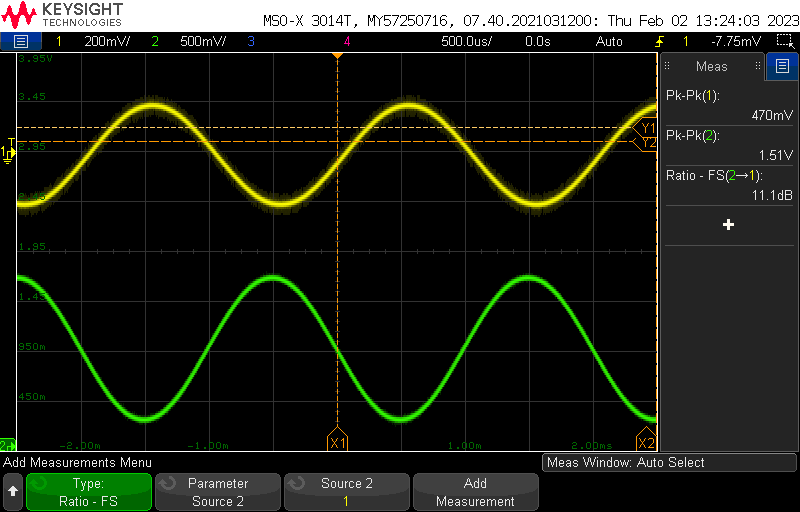
\includegraphics[scale=0.45]{scopeshot.png}
\end{center}

\newpage

\textbf{Step 6}\\
\indent The voltage gain $A_y$ is calculated using the following equation:

\begin{equation}
    A_y = \frac{v_{OUT}}{v_{IN}}
\end{equation}

which when used with the values measured by the oscilloscope, 

\begin{equation}
    A_y = \frac{1.51 V}{470 mV} \approx 3.212
\end{equation}

with percent error:

\begin{equation}
    \% error = \frac{measured - calculated}{calculted} = \frac{3.212 - 4}{4} \approx 20\% err.
\end{equation}


\textbf{Step 7}

The following is the frequency response analysis for the circuit between 1 Hz and 500 kHz. \\

\begin{center}
    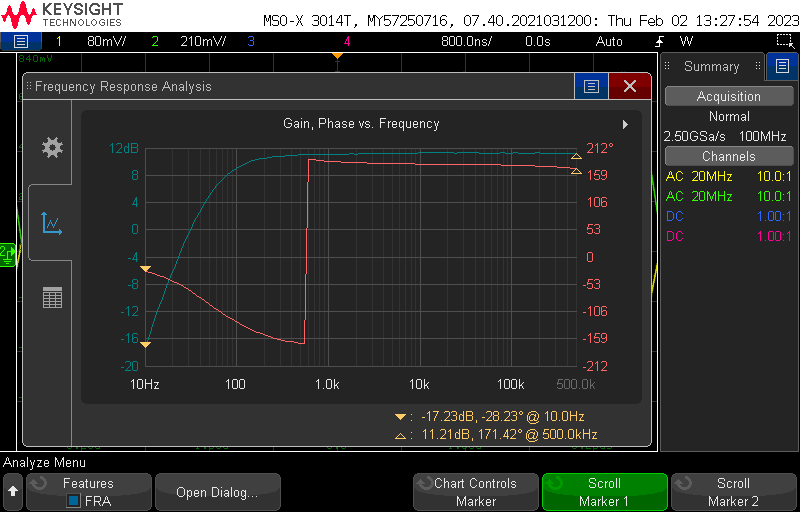
\includegraphics[scale=0.5]{frc.png}
\end{center}

\newpage

\textbf{Step 10}

The following is the largest signal amplitude that resulted in little distortion to the input signal.

\begin{center}
    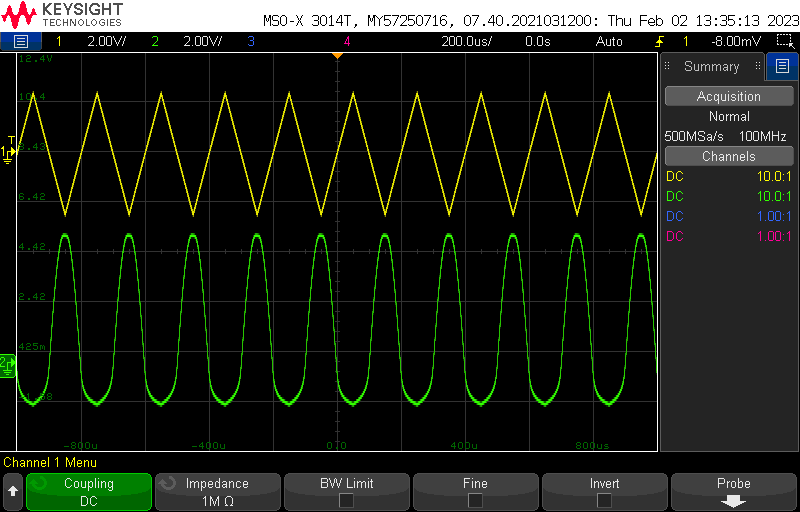
\includegraphics[scale=0.5]{tri.png}
\end{center}

The input voltage shown is 2.6V% INPUT VOLTAGE HERE
, which is approximately 1.6V% number here
above our design specification. Any signal larger than this experiences large distortion and clipping.

\subsection*{Conclusions}

In this task, we created an inverting amplifier using the ALD1106 chip and its enclosed N-type transistors. We created the amplifier 
as per the design specifications, and had a working amplifier with very little error in our design choices. 


\newpage

\printbibliography[title={\Large References}] %Prints out the bibliography sources that you have used in the document.

\end{document}